\chapter{Almacen}
\begin{justify}
    El Departamento de Almacén es una sección esencial dentro de la aplicación Telintec, diseñada para gestionar el inventario, registrar movimientos de productos y facilitar el control eficiente de materiales. A continuación, se describen las funciones de cada pestaña dentro de este departamento. 
\end{justify}
\begin{justify}
Estas pestañas permite la gestión detallada de los productos dentro del almacén. Las funcionalidades principales son: inventario, movimientos  y despacho de solicitudes de material
\end{justify}


\newpage
\pagestyle{fancy}

\section{Panel principal-\textit{Dashboard}}
\begin{justify}
    El Panel Principal del sistema Telintec es la interfaz inicial, mostrada en las figuras \ref{fig:dashboard}, que cada usuario ve después de iniciar sesión. Este panel está diseñado para adaptarse al rol y departamento del usuario, mostrando únicamente las funciones y herramientas autorizadas para su perfil. 
\end{justify}


\begin{figure}[ht!]
\centering
\begin{subfigure}{0.45\textwidth}
    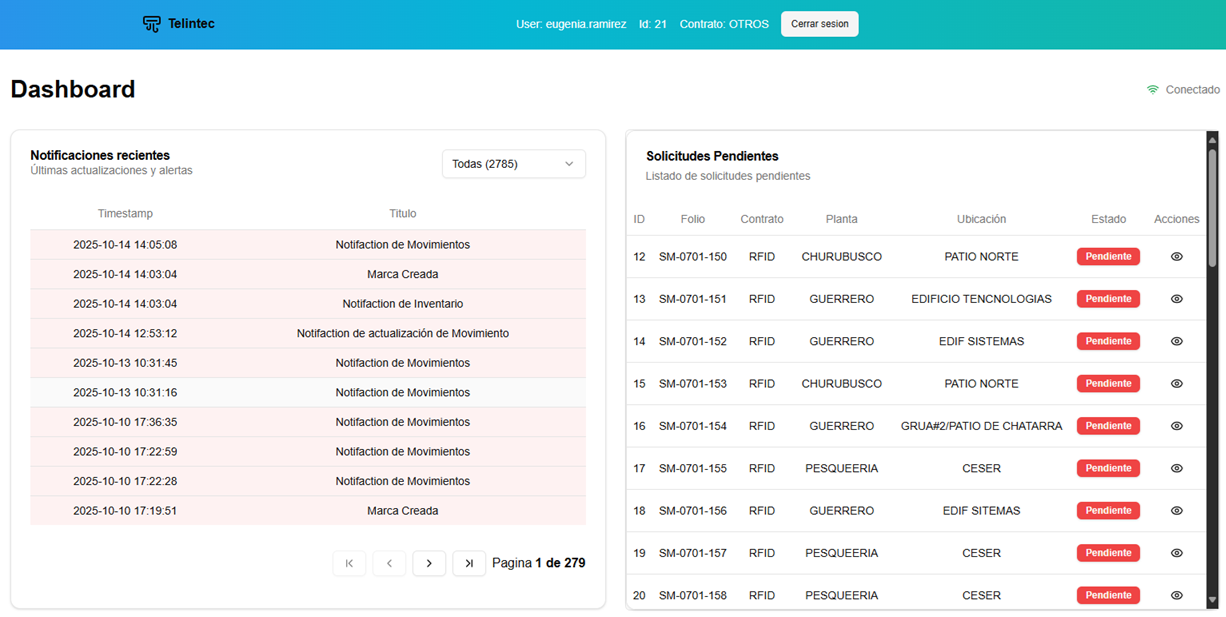
\includegraphics[width=\textwidth]{imgs/Almacen General/Dashboard/almacen_deahboard.png}
    \caption{Ventana de dashboard.}
    \label{fig:dash1}
\end{subfigure}
\hfill
\begin{subfigure}{0.45\textwidth}
    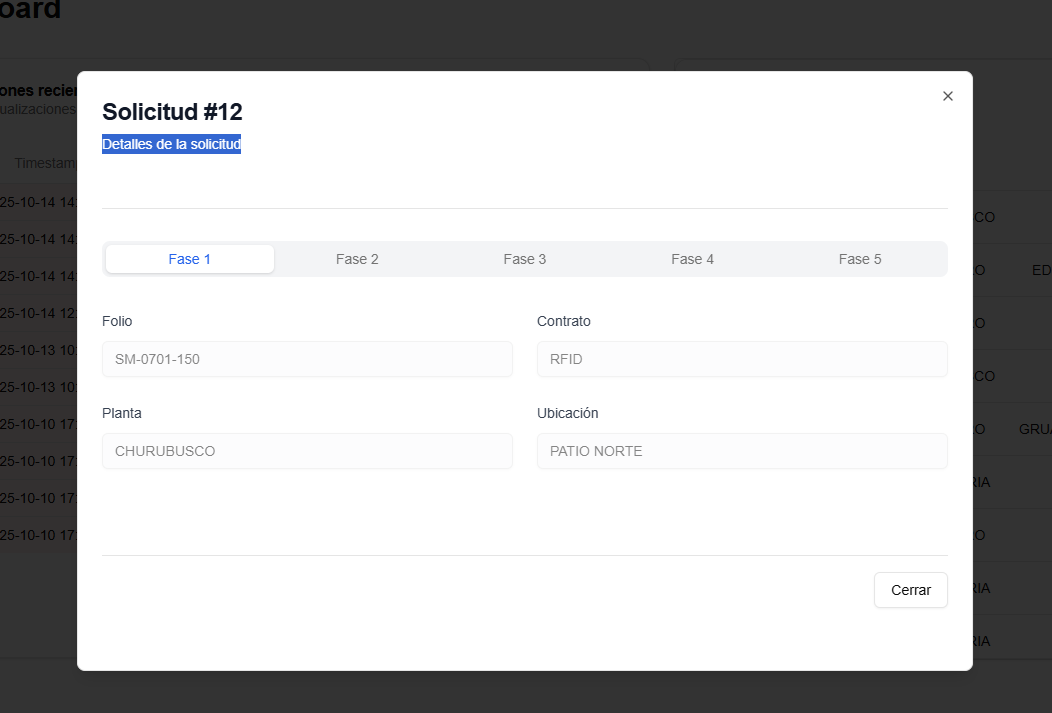
\includegraphics[width=\textwidth]{imgs/Almacen General/Dashboard/almacen_acciones.png}
    \caption{Acciones - Solicitudes pendientes.}
    \label{fig:dash2}
\end{subfigure}        
\caption{Panel de inicio.}
\label{fig:dashboard}
\end{figure}



\subsection{Características de la Pestaña Inicio} 

Una vez que el usuario inicia sesión, es redirigido automáticamente a su Dashboard, donde podrá visualizar: 
La pestaña "Inicio" del sistema Telintec ofrece diversas funcionalidades clave para el usuario:
\begin{itemize}
    \item \textbf{Notificaciones sobre el inventario:} En esta sección, podrás ver las notificaciones de las acciones realizadas en el inventario, como:
    \begin{itemize}
        \item \textbf{Creación de productos:} Se mostrará una notificación cuando se haya agregado un nuevo producto al inventario.
        \item \textbf{Eliminación de productos:} Aquí aparecerá una notificación si algún producto ha sido eliminado del inventario.
        \item \textbf{Actualización de productos:} Si algún producto ha sido actualizado (por ejemplo, cambios en la descripción, precio o cantidad), se mostrará una notificación indicando la acción realizada.
    \end{itemize}

    \item \textbf{Notificaciones de movimientos:} También se notifican los movimientos de productos dentro del sistema, tales como:
    \begin{itemize}
        \item \textbf{Entrada/Salida de productos:} Cuando los productos tengan salida y entrada, se registran en el inventario.
    \end{itemize}

    \item \textbf{Acciones destacadas:} Las acciones más importantes o urgentes aparecerán de manera destacada para que el usuario las identifique fácilmente.

    \item \textbf{Estadística:} En esta sección, se presentan datos clave sobre el estado y movimiento del inventario en forma de gráficos.
\end{itemize}

\subsubsection{Notificaciones relevantes}

En el caso de los empleados del departamento de Almacén, las notificaciones incluyen los diferentes estados de las Solicitudes de Material (SM), como solicitudes pendientes, en proceso o completadas. Estas notificaciones permiten a los usuarios mantenerse actualizados sobre las actividades clave de su área. 

\subsubsection{Menú principal personalizado}
El menú principal se adapta a las necesidades del usuario, presentando únicamente las opciones y pestañas autorizadas según su rol. Esto optimiza la experiencia del usuario y evita la confusión al eliminar elementos innecesarios. 

\subsection{Elementos comunes del dashboard }

El Dashboard incluye herramientas accesibles para todos los usuarios, como: 

\begin{itemize}
    \item Notificaciones: Indicadores visuales que alertan sobre acciones pendientes o eventos importantes relacionados con el departamento. 
    \item Menú Principal: Un acceso rápido a las principales pestañas y subpestañas relacionadas con las funciones del usuario. 
    \item Configuraciones: Opciones para actualizar el perfil del usuario, como el cambio de contraseña o ajustes de idioma. 
\end{itemize}


\subsection{Funcionalidades para almacén}

Para los empleados del almacén, el panel de inicio también incluye un acceso directo a las principales funciones operativas, organizadas en las siguientes pestañas: 

\begin{itemize}
    \item Inicio: Vista general de las notificaciones y acceso rápido a estados de Solicitudes de Material (SM). 
    \item Almacén: Inventario: Consulta y gestión de los productos disponibles en el almacén. 
    \item Movimientos: Registro y seguimiento de entradas y salidas de productos. 
    \item Procesamiento de SM: Herramienta para gestionar las solicitudes de material, desde su creación hasta su finalización. 
    \item Seguridad: Control y auditoría de accesos y actividades dentro del sistema. 
\end{itemize}

Este diseño modular asegura que cada usuario tenga acceso directo y simplificado a las funciones que necesita para cumplir sus tareas de manera eficiente y segura. 

 

\section{Inventario}
\begin{justify}
En esta pestaña, los usuarios pueden gestionar los productos en la base de datos, ya sea para dar de alta un nuevo producto, actualizar información existente o generar reportes.
\end{justify}
\begin{justify}
Registro de productos: Los usuarios pueden registrar nuevos productos en el sistema, incluyendo información clave como códigos, descripciones, categorías, proveedor y marca. La interfaz para estas operaciones se puede observar en las figuras \ref{fig:inventory}. Es importante resaltar que se puede agregar el código de barras manualmente. 
\end{justify}

\begin{figure}[ht!]
\centering
\begin{subfigure}{0.45\textwidth}
    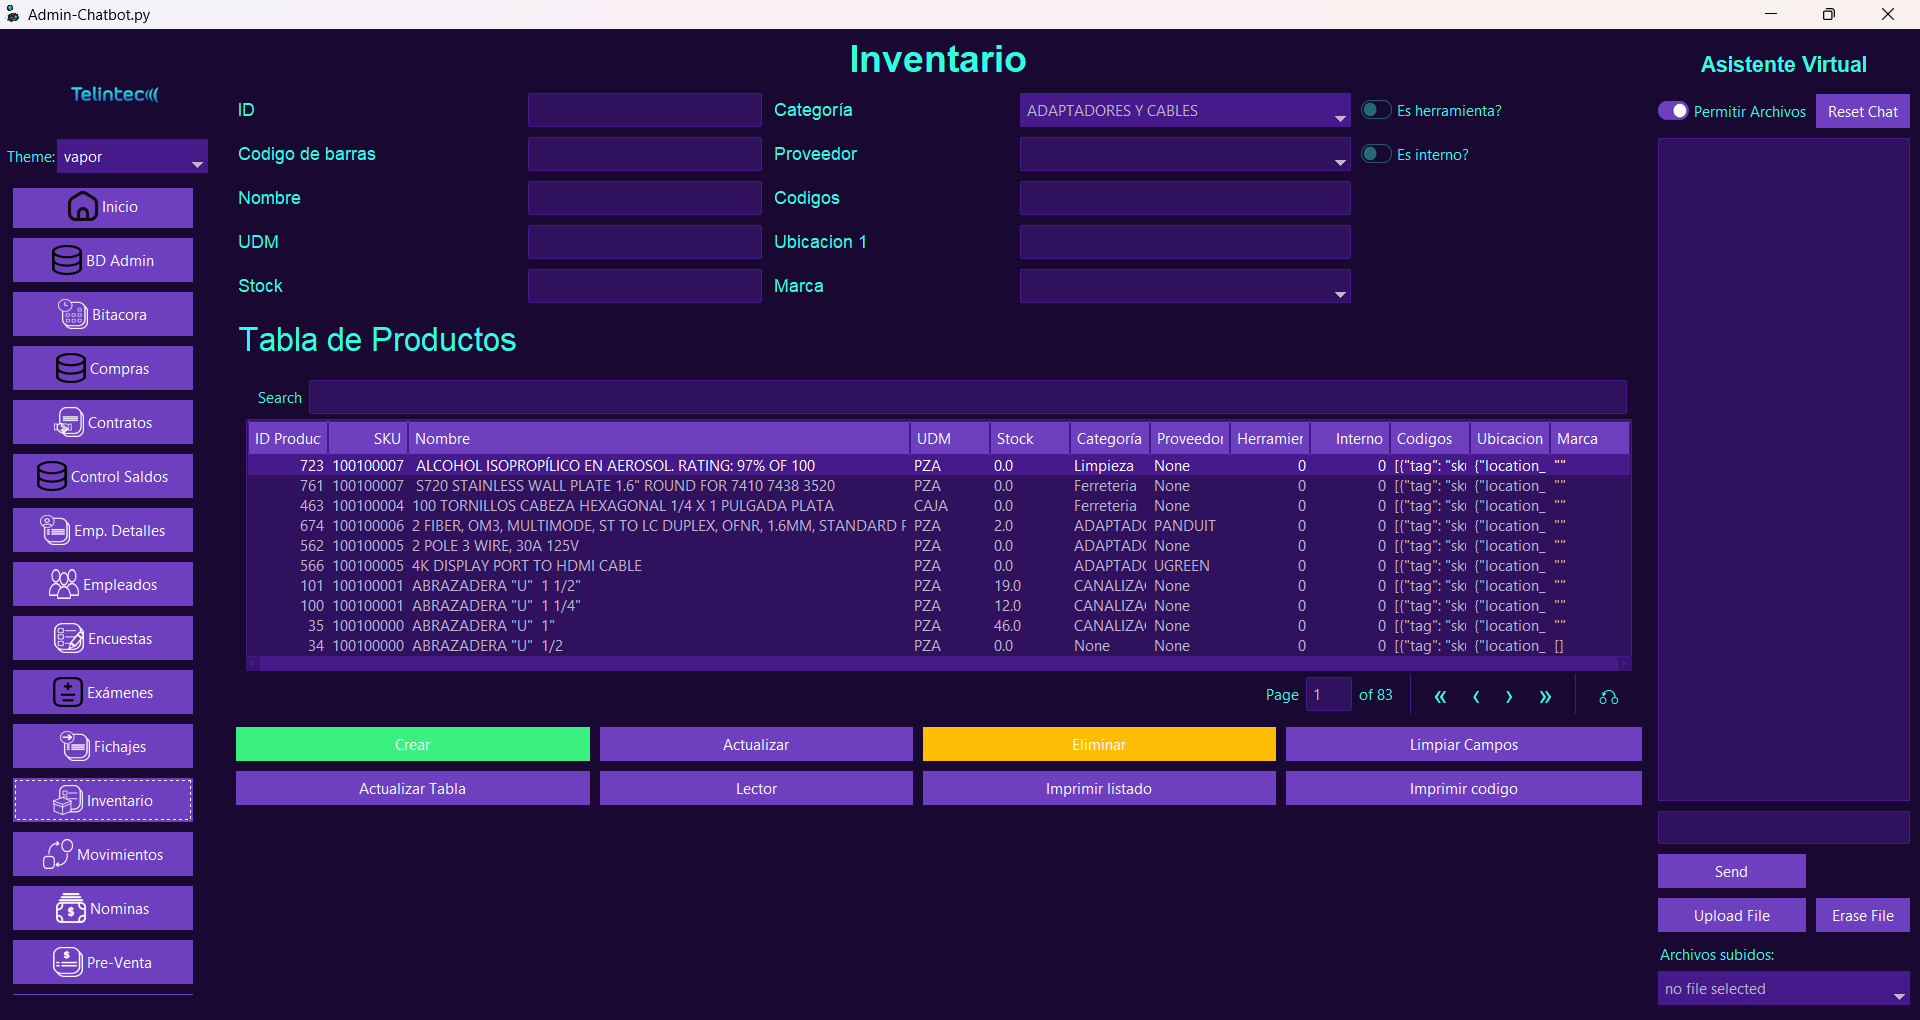
\includegraphics[width=\textwidth]{imgs/InventoryApp.png}
    \caption{Aplicación de escritorio.}
    \label{fig:invent1}
\end{subfigure}
\hfill
\begin{subfigure}{0.45\textwidth}
    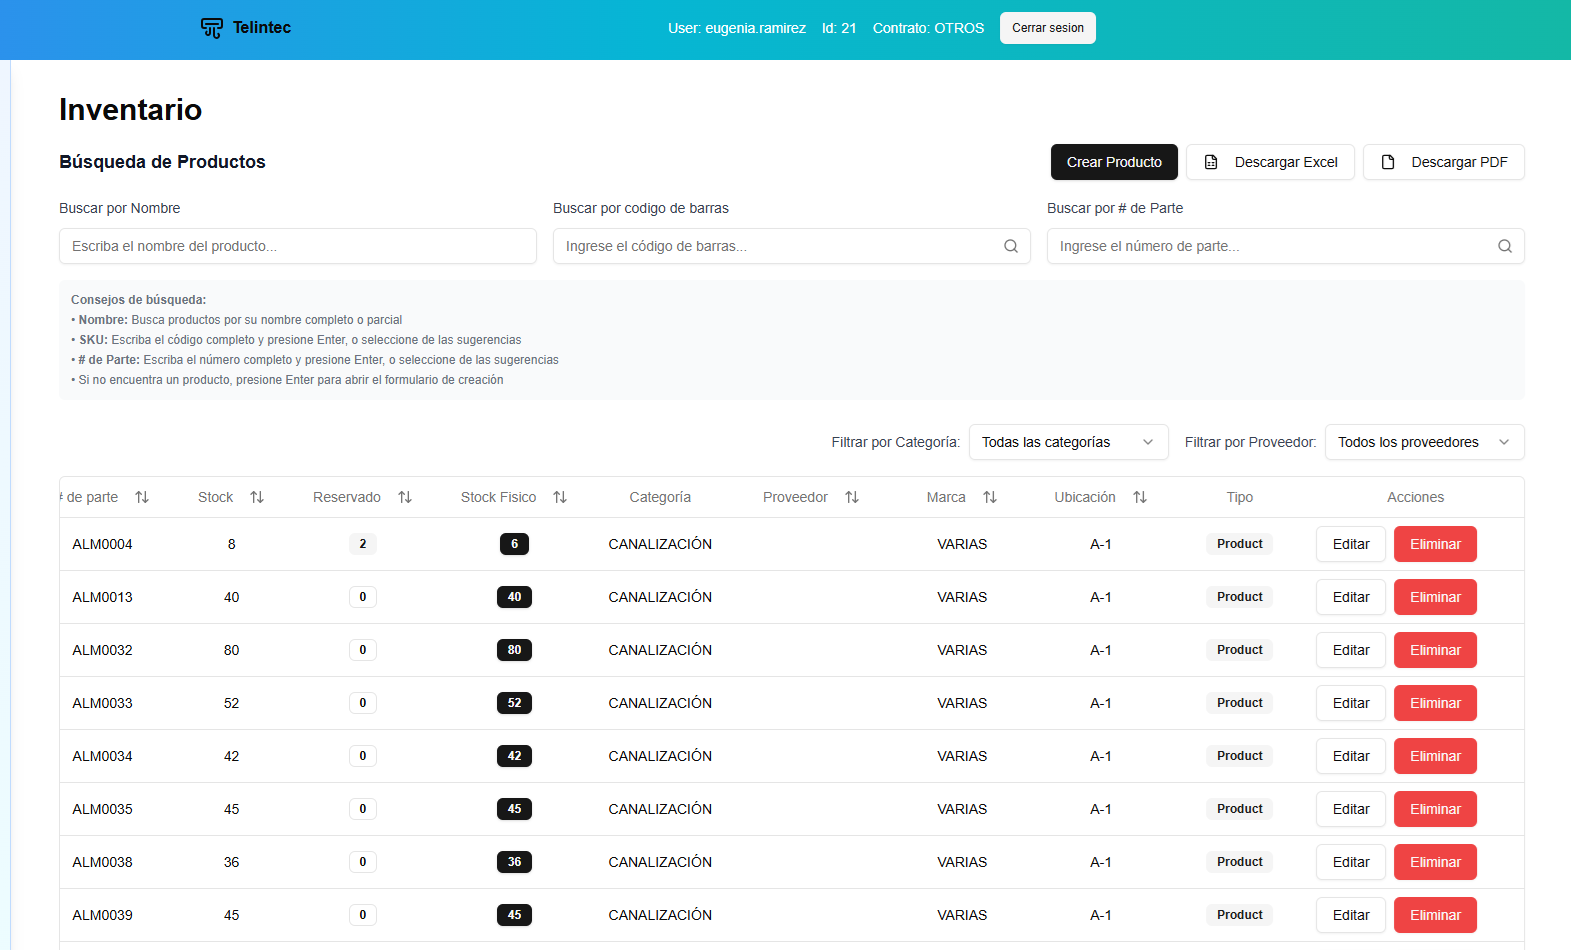
\includegraphics[width=\textwidth]{imgs/Almacen General/inventario/inventario_1_general.png}
    \caption{Apliación web.}
    \label{fig:invent2}
\end{subfigure}        
\caption{Ventana de inventario.}
\label{fig:inventory}
\end{figure}




Además, hay algunas restricciones del sistema que deben tomarse en cuenta: 

Al dar de alta un producto nuevo en el inventario, este puede registrarse mediante escáner o manualmente, y es obligatorio llenar todos los campos solicitados. Si se desea actualizar el stock de un producto existente, es necesario considerar que algunos productos antiguos pueden no tener información completa, como categoría, proveedor o códigos. Esto podría generar errores si no se actualizan estos campos junto con el stock. 

Es fundamental ser preciso al llenar el campo de “códigos”, ya que no se aceptan caracteres especiales. Funciones principales: La pestaña también permite realizar acciones clave como: 

\begin{itemize}
    \item Crear, actualizar y eliminar productos. 

    \item Actualizar la tabla donde se visualizan los productos. 

    \item Limpiar campos para facilitar el ingreso de nueva información. 

    \item Imprimir códigos, permitiendo crear y personalizar etiquetas de productos. 

    \item Utilizar el lector para escanear productos y registrar datos de manera rápida y precisa. 

    \item Consulta de existencias: Proporciona una vista actualizada de las existencias de productos disponibles, mostrando detalles como cantidades en almacén, ubicación y alertas de stock bajo. Además, el sistema permite visualizar los productos mediante una tabla, con la opción de buscarlos utilizando un buscador integrado. 
\end{itemize}

\section{Movimientos}

\subsection{Entradas}
Esta pestaña (Figura \ref{fig:ins}) se centra en la administración de los movimientos de inventario, ofreciendo las siguientes funciones: 

\begin{figure}[ht!]
\centering
\begin{subfigure}{0.45\textwidth}
    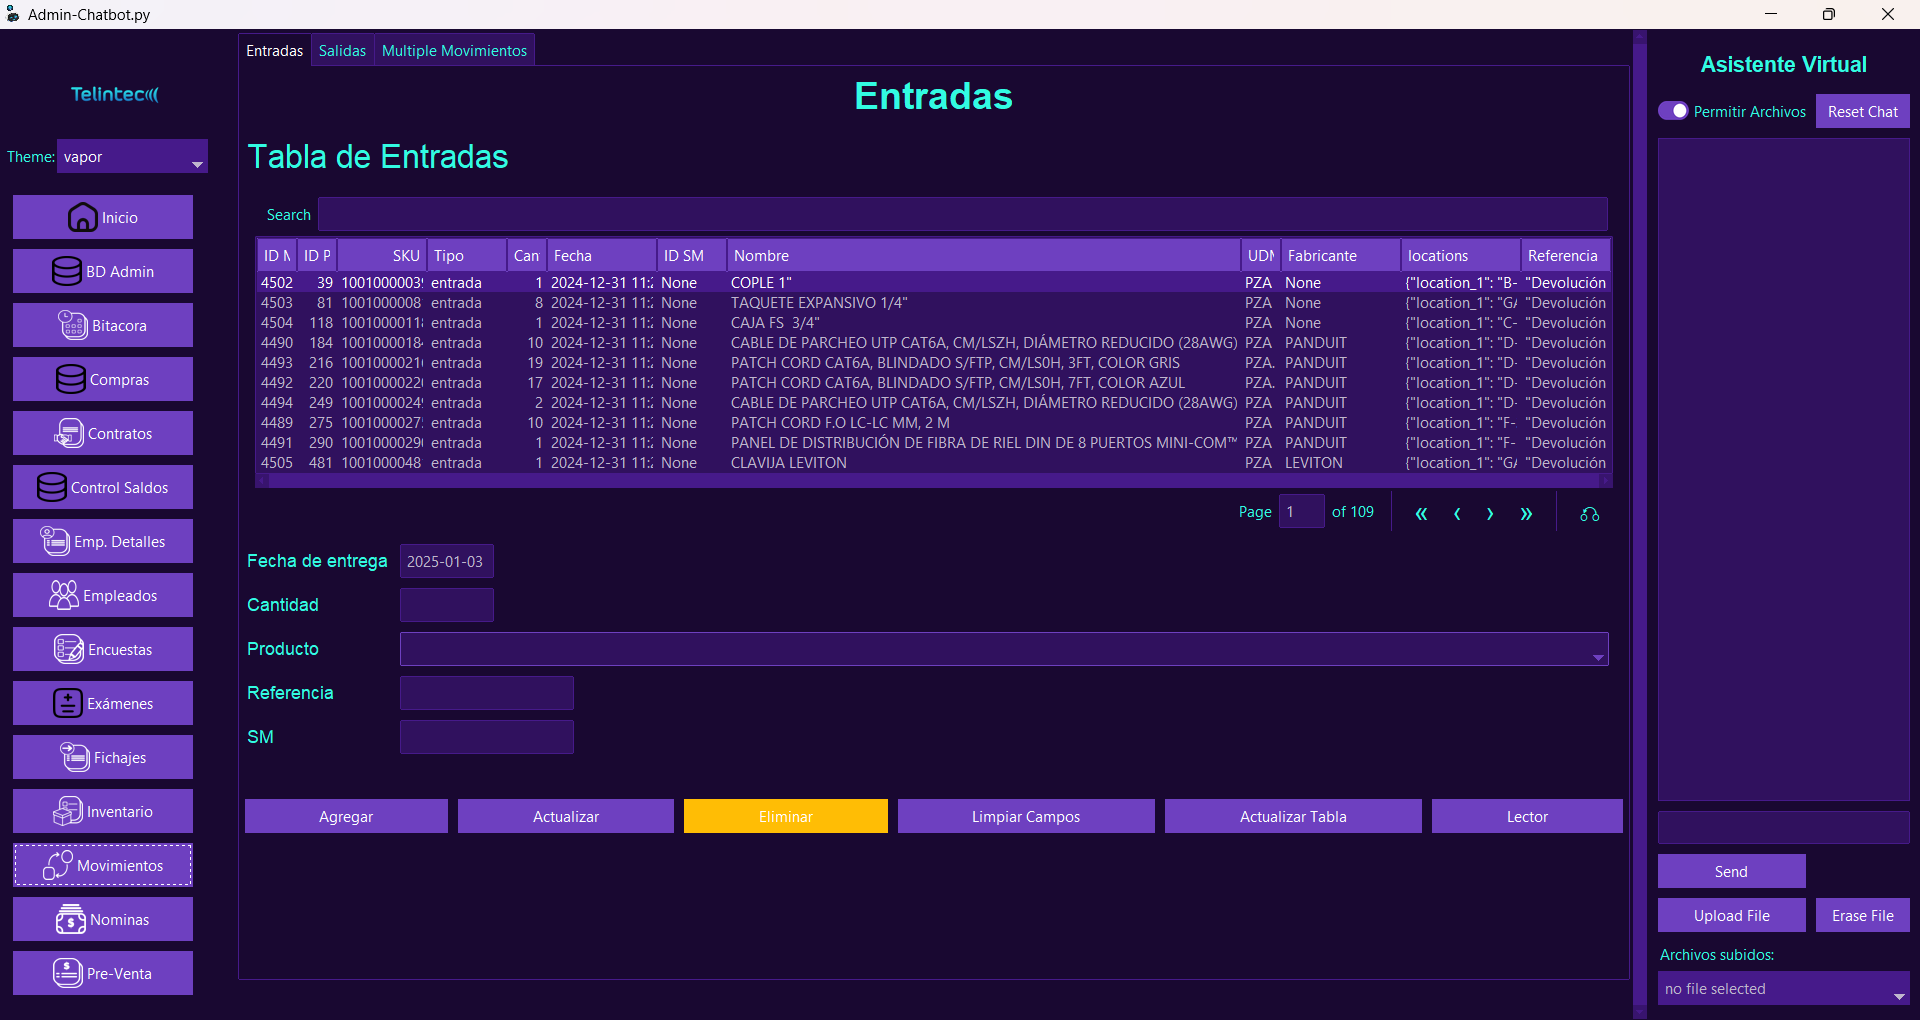
\includegraphics[width=\textwidth]{imgs/InsApp.png}
    \caption{Aplicación de escritorio.}
    \label{fig:ins1}
\end{subfigure}
\hfill
\begin{subfigure}{0.45\textwidth}
    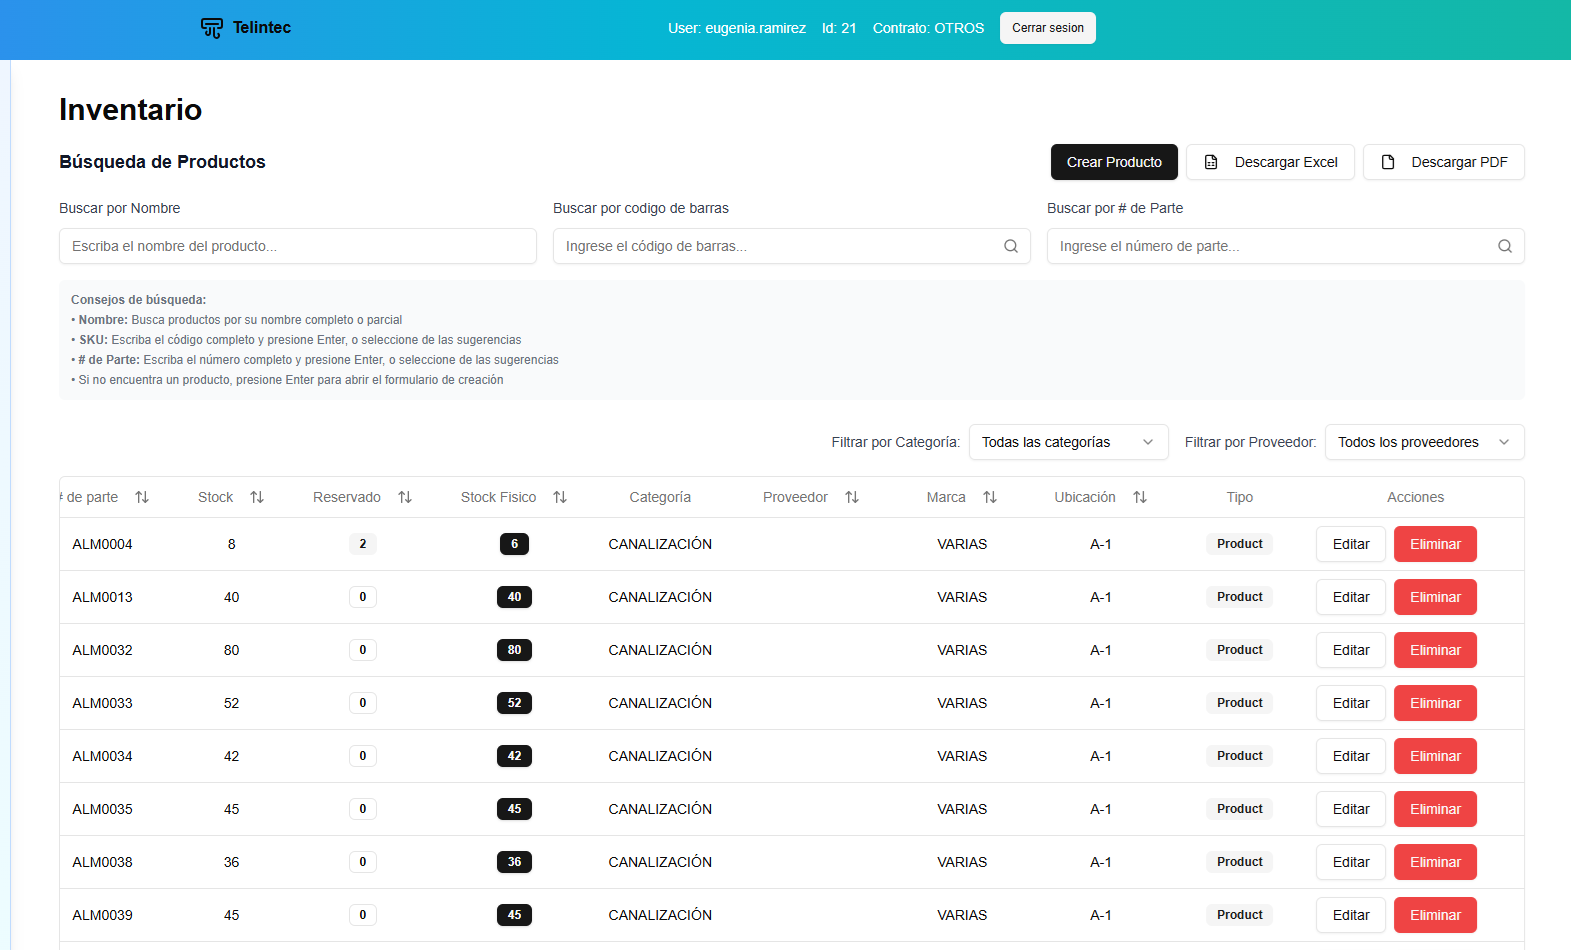
\includegraphics[width=\textwidth]{imgs/Almacen General/inventario/inventario_1_general.png}
    \caption{Apliación web.}
    \label{fig:ins2}
\end{subfigure}        
\caption{Ventana de creación de entradas.}
\label{fig:ins}
\end{figure}



Aquí, se permite registrar la recepción de productos en el inventario, ya sea por compras, devoluciones o ajustes. Visualiza los productos y ofrece las opciones de agregar una nueva entrada, actualizarla o eliminarla. Incluye un lector de código de barras para escanear los productos existentes a los cuales se desea dar entrada. 
\textbf{Importante}: No es posible crear productos directamente desde esta opción de entrada. 

\subsection{Salidas}

En esta interfaz (Figura \ref{fig:outs}), se facilita el registro de productos que salen del almacén, ya sea por ventas o devoluciones de clientes. Puedes crear, actualizar o eliminar una salida, y también hacerlo utilizando el lector de código de barras, simplemente escaneando el producto y completando los campos requeridos. 

\begin{figure}[ht!]
\centering
\begin{subfigure}{0.45\textwidth}
    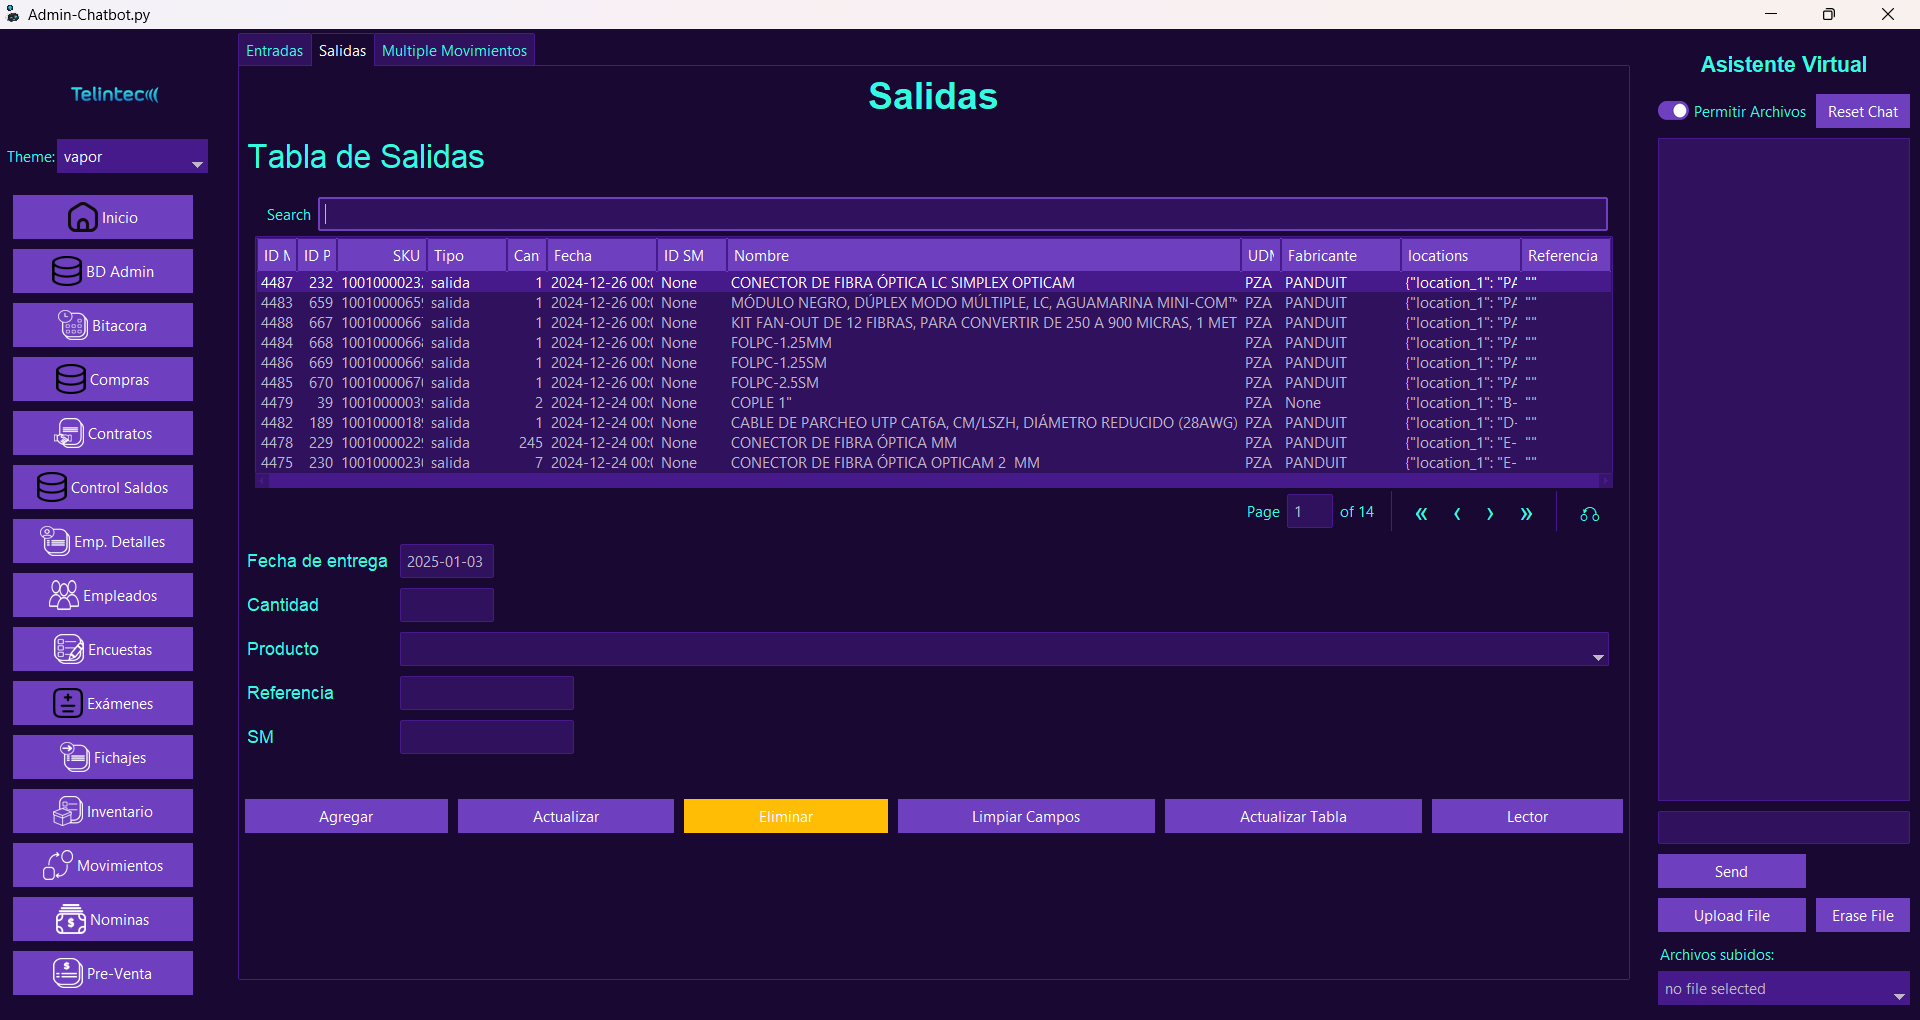
\includegraphics[width=\textwidth]{imgs/OutsApp.png}
    \caption{Aplicación de escritorio.}
    \label{fig:outs1}
\end{subfigure}
\hfill
\begin{subfigure}{0.45\textwidth}
    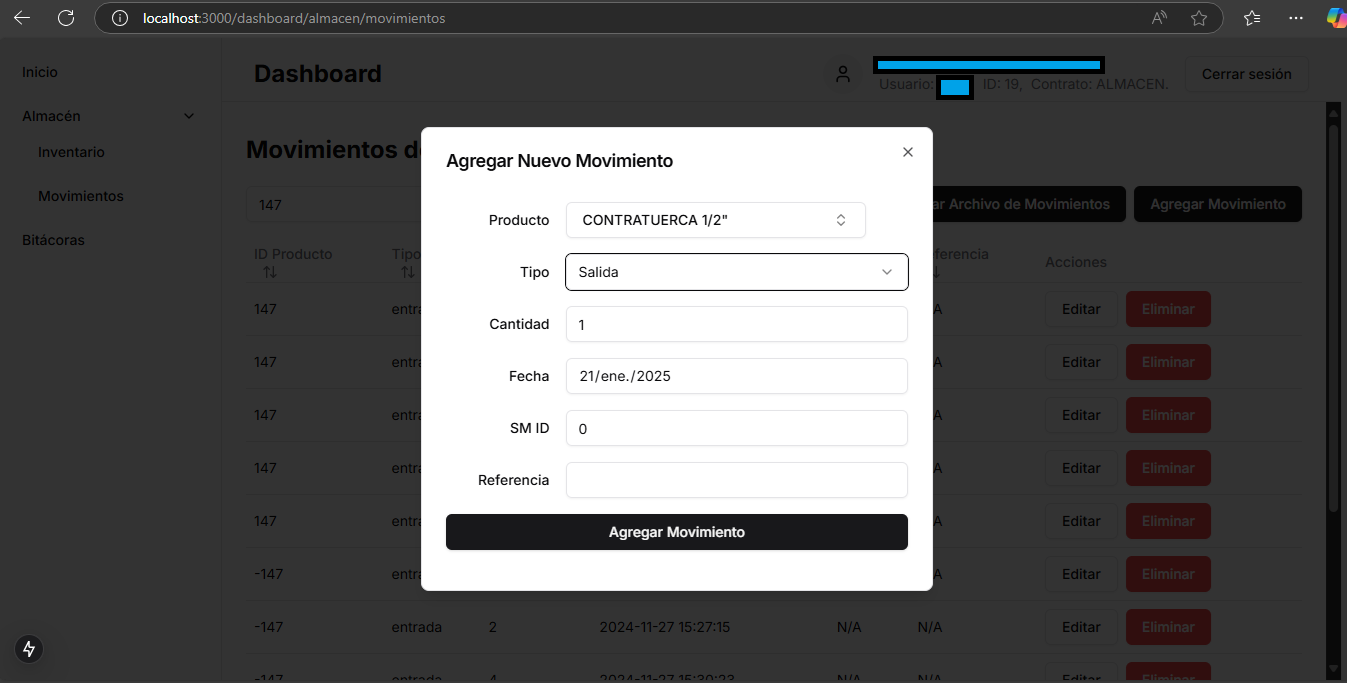
\includegraphics[width=\textwidth]{imgs/OutsWebApp.png}
    \caption{Apliación web.}
    \label{fig:outs2}
\end{subfigure}        
\caption{Ventana de inventario.}
\label{fig:outs}
\end{figure}

\textbf{Consideración}: Algunos productos más antiguos en el sistema tienen restricciones al intentar actualizar el stock. Si es necesario, deberás actualizar también nuevos campos que se añadan a petición de administración. 

\subsection{Movimientos múltiples} 
\begin{figure}[ht!]
\centering
\begin{subfigure}{0.45\textwidth}
    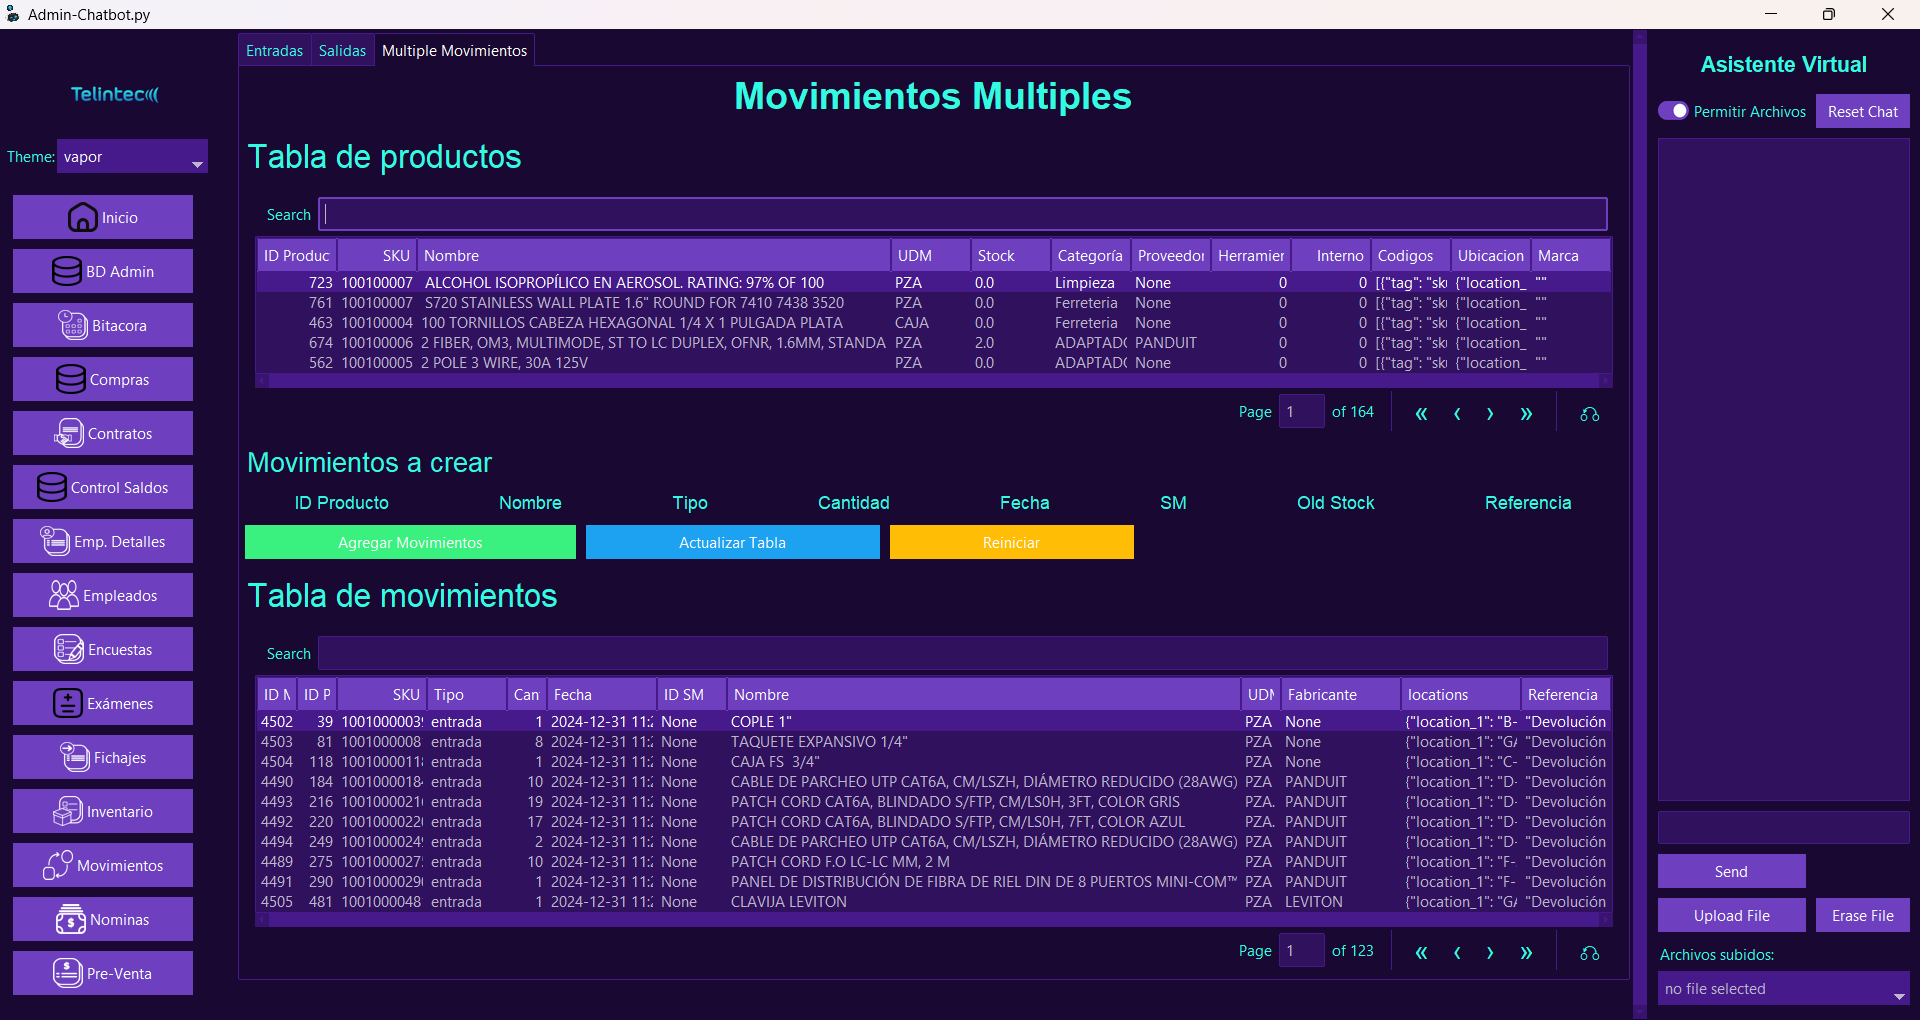
\includegraphics[width=\textwidth]{imgs/MultipleMovesApp.png}
    \caption{Aplicación de escritorio.}
    \label{fig:multimoves1}
\end{subfigure}
\hfill
\begin{subfigure}{0.45\textwidth}
    
\includegraphics[width=0.5\textwidth]{imgs/no-image.png}
    \caption{Apliación web.}
    \label{fig:multimoves2}
\end{subfigure}        
\caption{Ventana de ingreso de multiples movimientos.}
\label{fig:multimoves}
\end{figure}

Esta  interfaz (Figura \ref{fig:multimoves}) opción permite crear entradas y salidas simultáneamente para varios productos, los cuales se agregarán en forma de lista. El campo \textit{Old Stock} es solo una etiqueta visual para que puedas ver el stock actual. \textbf{No deberás modificar este campo.} 

\section{Solicitudes de Material}

Esta pestaña está diseñada para facilitar el proceso de solicitud y aprobación de materiales dentro de la organización. Sus funcionalidades incluyen: 

Creación de solicitudes: Permite a los usuarios generar solicitudes de material de manera rápida, especificando detalles como cantidades requeridas, razones de uso y fechas necesarias. 

Aprobación y seguimiento: Los administradores pueden aprobar o rechazar solicitudes y realizar un seguimiento de su estado hasta la entrega final. 

\section{Escaner}

La pestaña del escáner está enfocada en optimizar el registro de movimientos de inventario mediante el uso de tecnología de códigos de barras. Para la aplicación de escritorio se despliega una ventana extra donde se realizan las operaciones del lector. Las funciones disponibles son: 

\begin{figure}[ht!]
\centering
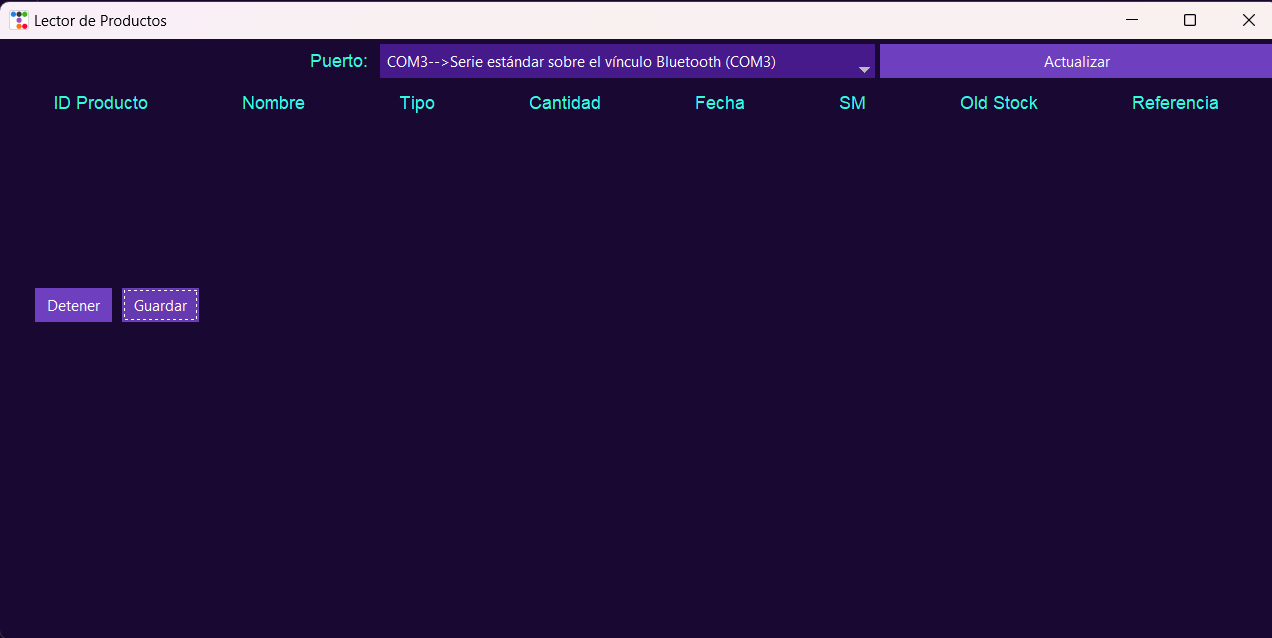
\includegraphics[width=0.7\textwidth]{imgs/LectorApp.png}
\caption{Ventana emergente para funcines del lector.}
\label{fig:lecotr}
\end{figure}

Permite a los usuarios registrar entradas y salidas de manera rápida y precisa escaneando los códigos de barras de los productos. Esto facilita la gestión del inventario de manera eficiente y sin errores manuales.

\textbf{¿El escáner se desconfiguró?} Sigue estos pasos:
\begin{enumerate}
    \item Verifica la conexión: Asegúrate de que el escáner esté correctamente conectado al dispositivo. Si es inalámbrico, comprueba que esté dentro del rango de la red o que la batería esté cargada. 

    \item Reinicia el escáner: Apaga el escáner y vuélvelo a encender para restablecer su configuración. 

    \item Reconfigura el escáner: 
    \begin{itemize}
        \item Escanea el código de configuración que aparece en el manual del escáner para restablecer los ajustes predeterminados.
        \item Puedes acceder al manual desde el 
        \href{https://drive.google.com/file/d/1OsTJD1-Hbvdd9wIGknSJqKVfENMQDajR/view?usp=sharing.}{\emph{enlace}}. 
        \item Este manual incluye los códigos necesarios y las instrucciones detalladas para la configuración.
    \end{itemize}
    \item Verifica la configuración del software. Asegúrate de buscar en tu dispositivo el administrador de dispositivos los puertos (COM) y poder ver si el escáner ya es reconocido por el dispositivo.

    \item Consulta la guía de solución de problemas. Si el escáner sigue sin funcionar correctamente, consulta la guía de solución de problemas para verificar posibles errores de lectura o ajustes necesarios. 
\end{enumerate}